\subsection{Use-case Example: Deuteron}
Deuteron $d$ has total spin $J = 1$, as each nucleon is half-spin particles. We also assume that the ground state has $L = 0$. The total state is therefore $^{3}S_1$. This predicts a magnetic dipole moment as the sum of the magnetic dipole moments of the proton and neutron. This is because we only take into account their intrinsic spins. This is close to what experiment show, but not quite. The reason for this discrepancy is that $L$ can be 2. This gives us the $^{3}D_1$ state. This explains the difference. For bound states, $L$ is only approximately a good quantum number. 

\section{Quark Model}
\subsection{Hadron Spectroscopy}
If we assume the following:
\begin{itemize}
    \item $L$ and $S$ are good quantum numbers. 
    \item Quarks have spin $1/2$.
    \item Mesons are $q \bar{q}$, baryons are $qqq$, with $q ∈ \left\{u, d, s, c, b\right\}$
    \item Lightest mesons states have $L = 0$. 
    \item Lightest baryon states have $L_{12} = L_3 = 0$
\end{itemize}
\subsubsection{Mesons}
\begin{itemize}
    \item Two possible spin states: $S = 0$ and $S = 1$.
    \item For $L = 0$ and $J = S$ we can have $^{1}S_0$ and $^{3}S_1$ states.
    \item This predicts two ground states with different spins. Things are more complicated with $L = 1$. 
    \item For $L = 1$ and $J = L - 1, \ldots  L +1$ if $S = 0$ or $J = L$ if $S = 0$. 
    \item For lighter mesons we have $L = 0$ and $S = 1$, for the lightest we have $S = 0$, as well. For heavier mesons we have $L = 1$. 
    \item The heavier ones have a shorter lifespan. 
\end{itemize}

\subsubsection{Baryons}
\begin{itemize}
    \item 3 spin-$1 / 2$ quarks so that $S = 1 / 2$ or $3 / 2$. 
    \item For $L = 0$ we have 2 states $^{2}S_{1 / 2}$ and $^{4}S_{3 / 2}$. 
    \item for $L = 1$ it again gets more complicated. We have 5 $P$-states and 6 $D$-states. 
    \item Light $S$-states include $p, n, Λ, Λ_{c}, Λ_{b}$. We expect to find heavier and more unstable states for $S = 3 / 2$. 
\end{itemize}

\subsection{Intrinsic Parity of Hadrons}
\begin{itemize}
    \item $P_{\text{meson}} = P_a P_{\bar{b}} (-1)^{L} = (-1)^{L+1}$. 
    \begin{itemize}
        \item Low-mass mesons with $L=0$ predicted to have $P = -1$, consistent with observations of $π$, $K$, $D$
    \end{itemize}
    \item $P_{\text{baryon}} = P_a P_b P_c (-1)^{L_{12} + L_3}$. 
    \item $P_{\text{anti-baryon}} = P_{\bar{a}} P_{\bar{b}} P_{\bar{c}} (-1)^{L_{12} + L_3} = (-1)^{L_{12} + L_3 + 1}$.
    \begin{itemize}
        \item Low bass baryons with $L_{12} = L_3 = 0$ predicted to have $P = +1$, with anti-baryons having $P = -1$.
    \end{itemize}
\end{itemize}

\subsection{Charge Conjugation (particle $↔$ anti-particle)}
\begin{itemize}
    \item The parity operator $\hat{C}$ changes particle to anti-particle and vice versa.
    \item Both $C$-parity and $P$-parity are conserved during strong and electromagnet interactions.
    \item Some particles, like the photon, are their own anti-particle. They are eigenstates of the operator $\hat{C}$.
    \item Other states have distinct anti-particles. They are not eigenstates of the operator $\hat{C}$.
    \item C-parity eigenstates can be constructed by particle-antiparticle paris that are symmetric or anti-symmetric under exchange of the particles $a \leftrightarrow \bar{a}$. This could be done as follows: 
    \begin{equation}
      \hat{C} \ket{a Ψ_1, \bar{a}Ψ_2} = \ket{\bar{a}Ψ_1, aΨ_2} = ± \ket{aΨ_1, \bar{a}Ψ_2}
    \end{equation} 
    \item An example could be the pion. 
    \begin{equation}
      \hat{C} \ket{π^{+} π^{-} ; L} = (-1)^{L} \ket{π^{-} π^{+} ; L}
    \end{equation}
\end{itemize}

\subsubsection{C-parity of pion $π^{0}$}
\begin{itemize}
    \item The pion often decays to two photons $\pi^{0} \rightarrow γγ$. The photons have their own C-parity, but as a unit they must have the same C-parity as the pion, $\hat{C} π^{0} = +1$. The question is, does the photons each have $C = +1$ or $C = -1$?
    \item As we never have observed a decay of the pion to three photons, we can conclude that the photons must have $C = -1$.
\end{itemize}

\subsubsection{C-parity of $η$}
\begin{itemize}
    \item Neutral spin-+ mesons with great mass of 558 MeV and spacial parity $\hat{P} η = -1$. 
    \item $B(η → γγ)$ happens $39\%$ of the time. We know the photons have $C = -1$, so the $η$ must have $C = +1$.
    \item $B(η → π^{0} π^{0} π^{0})$ happens $33\%$ of the time. The pions have $C = +1$, so the $η$ must have $C = -1$.
    \item $B(η → π^{+} π^{-} π^{0})$ happens $23\%$ of the time. Applying the C-parity operator to the pions as below:
    \begin{equation}
        \hat{C} \ket{π^{+}p_1, π^{-}p_2, π^{0}p_2} = \ket{π^{-}p_1, π^{+}p_2, π^{0}p_3} 
    \end{equation}
    This predicts that the momentum of the pions must be indistinguishable. 
    \item We can then predict why the probability of $B(η → π^{0} π^{0}) = 0\%$. It fulfills the conservation of C-parity, but not the spacial parity. One needs to check both attributes. 
\end{itemize}

\subsubsection{C-parity of Spin-1/2 Fermions}
General formula:
\begin{equation}
  \hat{C} \ket{f \bar{f}; J, L, S} = (-1)(-1)^{S + 1}(-1)^{L} \ket{f \bar{f}; J, L, S} = (-1)^{L + S} \ket{f \bar{f}; J, L, S}
\end{equation}
\begin{itemize}
    \item This comes from $(-1)^{L}$ from the space inversion. 
    \item $(-1)$ comes from the exchange of fermion-antifermion (QFT).
    \item The exchange of the spin wavefunction gives rise to the $(-1)^{S + 1}$ term.
\end{itemize}

\subsection{Quantum Numbers}
Important quantum numbers, where the subscripts stands for strangeness $s$, charm $c$, bottomness $b$, topness $t$ and quark $q$, respectively. They may or may not be conserved during weak interactions.:
\begin{itemize}
    \item $S = - (N_s - N_{\bar{s}})$
    \item $C = + (N_c - N_{\bar{c}})$
    \item $\tilde{B} = - (N_{b} - N_{\bar{b}})$
    \item $T = + (N_t - N_{\bar{t}})$
    \item $B ≡ N_q / 3 = \left(N_q - N_{\bar{q}}\right) / 2$
    \item Hypercharge $Y = B + S + C + \tilde{B} + T$
    \item Isospin $I_3 = \frac{1}{2}(N_u - N_d) - \frac{1}{2}(N_{\bar{u}} - N_{\bar{d}})$
    \item $I_3 = Q - Y / 2$, with $Q$ being the Coulomb charge.
    \item Full table of quark quantum numbers can be found in \cref{fig: quark_quantum_numbers}. The anti-quarks have the opposite quantum numbers, with the exception of Isospin $I$. $I_3$ is the opposite as well. 
    \item These numbers can be used as a basis for spanning out the possible states of quarks. 
\end{itemize}
\begin{figure}[h!]
\centering
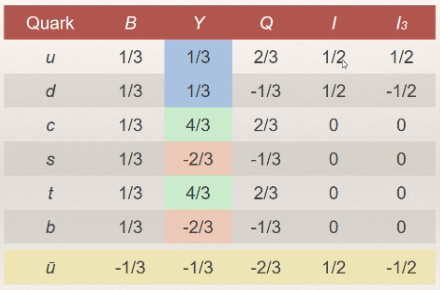
\includegraphics[width = .5\textwidth]{quark_quantum_numbers.png}
\caption{Table of quark quantum numbers.}
\label{fig: quark_quantum_numbers}
\end{figure}

\subsubsection{Hadrons With $C = \tilde{B} = T = 0$}
\begin{itemize}
    \item Isospin states: 
    \begin{itemize}
        \item $\frac{1}{2} + \frac{1}{2} = (0,1)$
        \item $\frac{1}{2} + \frac{1}{2} + \frac{1}{2} = (0,1) + \frac{1}{2} = \frac{1}{2}, \frac{1}{2}, \frac{3}{2}$
    \end{itemize}
    \item Table of isospin states can be found in \cref{fig: isospin_states}.
    \begin{figure}[h!]
    \centering
    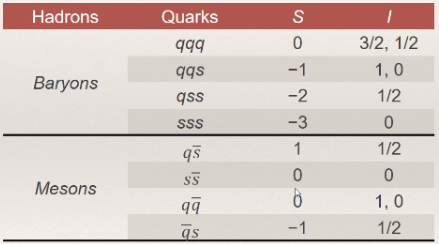
\includegraphics[width = .5\textwidth]{isospin_states.png}
    \caption{Table of isospin states.}
    \label{fig: isospin_states}
    \end{figure}
    
\end{itemize}

\paragraph{Example: $Σ^{+}$}
\begin{equation}
  K^{-} p → Σ^{+} π^{-}
\end{equation}
\begin{itemize}
    \item Looking at their quantum on the left-hand side we find that $S = -1$, $B = 1$, $C = \tilde{B} = T = 0$. The right-hand side has $S = 0$, $B = 0$, $C = \tilde{B} = T = 0$ and our $Σ^{+}$. For the quantities to be conserved we infer the values of the other $Σ^{+}$, which must be $S = -1$, $B = +1$, $C = \tilde{B} = T = 0$.
    \item Then we find the Isospin using $I_3 = Q - \frac{Y}{2}$ which gives $I_3 = 1$. We have two choices for $I$, either $0$ or $1$. As $I_3 = 1$, we must have $I = 1$ as well. This gives a $\ket{I, I_3} = \ket{1,1}$ state. 
    \item There must be two other charged members of the iso-triplet with $I_3 = 0, -1$, giving $Q = I_3 + Y / 2 = 0,-1$, as number of states are at least $N = 2 ⋅ I + 1$. We know from experiment this is $K^{0}$ and $K^{+}$. 
    \item The model predicted 3 states. There are no double charged $Σ^{--}$ or $Σ^{++}$ states. 
\end{itemize}

\subsubsection{Light Baryon Multiplets $L_{12} = L_3 = 0$ (\cref{fig: light_baryon_multiplets})}
\begin{figure}[h!]
\centering
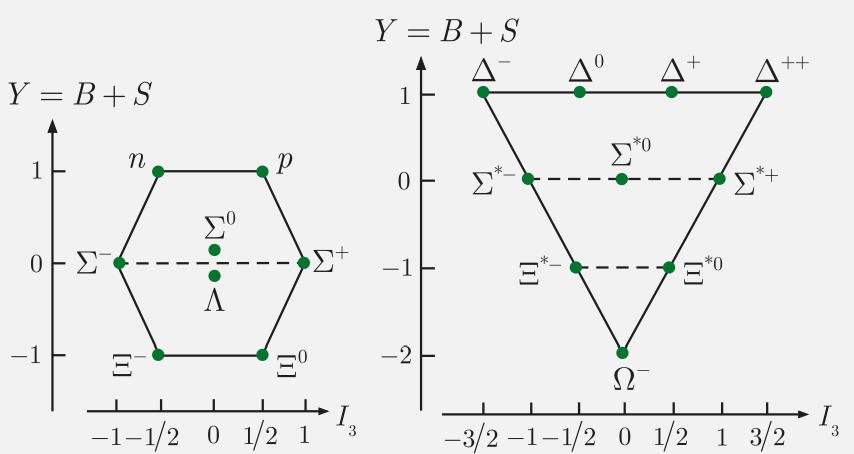
\includegraphics[width = .75\textwidth]{light_baryon_multiplets.png}
\caption{Different light baryon multiplets. Spin-1/2 particles to the left, and spin-3/2 particles to the right. On the bottom right, there should be a $Ω^{-}$.}
\label{fig: light_baryon_multiplets}
\end{figure}

\subsubsection{Light Mesons Nonets (\cref{fig: light_mesons_nonets,fig: quark_content})}





\begin{figure}[hb!]
\centering
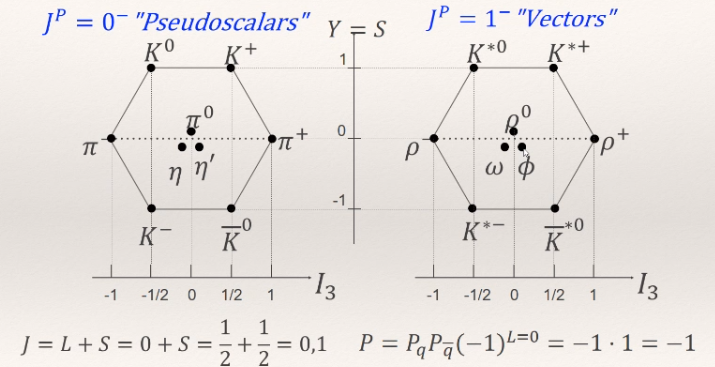
\includegraphics[width = .75\textwidth]{light_mesons_nonets.png}
\caption{Different light meson nonets. Pseudoscalar means that their wavefunction has some sign associated with it}
\label{fig: light_mesons_nonets}
\end{figure}

\begin{figure}[hb!]
\centering
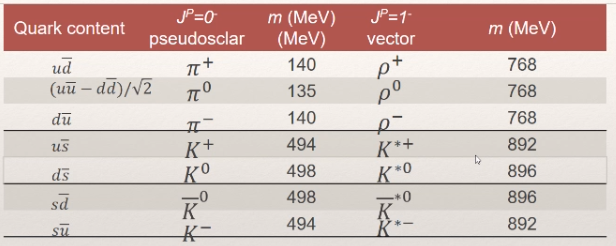
\includegraphics[width = .75\textwidth]{quark_content.png}
\caption{Quark content of different mesons and baryons. Some are unambiguously known, while others like $η$ and $\bar{η}$ are linear combinations of $u \bar{u}$, $d \bar{d}$ and $s \bar{s}$.}
\label{fig: quark_content}
\end{figure}



\subsection{Baryon Quark-Spin Wave Functions}
\begin{itemize}
    \item If we assume the wavefunctions $Ψ = ψ_{\text{space}}⋅ χ_{\text{spin}}$ of identical quarks are symmetric (while they are fermions), although this conflicts with the Pauli exclusion principle (for now). 
    \item As orbital angular momentum is 0, the the spin part must also be symmetric. This does not allow $S = 0$, as it would mean an anti-symmetric spin wavefunction. $S$ can only be $1$. 
    \item The only way to make $Δ^{++}(uuu)$, $Δ^{-}(ddd)$ and $Ω^{-}(sss)$, have symmetric spin is to have all three spins in parallel. This gives $J = 3 / 2$, and not $J = 1 / 2$
    \begin{itemize}
        \item For either $uud$, or $udd$, the two like quarks must be in $S = 1$, giving $↑_{a}↑_{a}↑_{b}$ or $↑_{a}↑_{a}↓_{b}$. The total $S = 1 + \frac{1}{2} = \frac{1}{2}, \frac{3}{2}$. 
        \item For protons and neutrons this gives $n,p → J = \frac{1}{2}$, and for $Δ^{+}, Δ^{0}$ we have $J = \frac{3}{2}$.
    \end{itemize}       
    \item For $uss$ and $dss$, the $ss$ must be in $S = 1$. When adding the third quark, the total $S = 1 + \frac{1}{2} = \frac{1}{2}, \frac{3}{2}$.
    \begin{itemize}
        \item For $Ξ^{-}$ and $Ξ^{0}$ with $J = 1 / 2$ and $Ξ^{*-}$ wnd $Ξ^{*0}$ with $J = 3 / 2$.
    \end{itemize}
    \item For $uus$ and $dds$, the non-$s$ must be in $S = 1$. When adding the third quark, the total $S = 1 + \frac{1}{2} = \frac{1}{2}, \frac{3}{2}$.
    \begin{itemize}
        \item For $Σ^{-}$ and $Σ^{+}$ with $J = 1 / 2$ and $Σ^{*-}$ and $Σ^{*+}$ with $J = 3 / 2$.
    \end{itemize} 
    \item For the $uds$-state we have $ud$ in $S = 1$, by isospin symmetry. the last $s$-quark gives $Σ^{0}$ with $J = 1 / 2$ and $Σ^{*0}$ with $J = 3 / 2$.
    \item An isospin-orthogonal $uds$ state has the $ud$ in $S = 0$. When adding the $s$ quark gives only one state of $S = 1 / 2$. This gives us $Λ$ with $J = 1 / 2$. Notice there is no excited state of $Λ$, as seen in \cref{fig: light_baryon_multiplets}.
\end{itemize}

